\begin{tcolorbox}[colback=white,colframe=black,opacityframe=0,colbacktitle=black,title={\textbf{Problem 7 [\examproblemweight\ points]}}]
\begin{enumerate}[label=(\alph*)]
	\item \textbf{(2 points)} Solve the following equation: $|x-\f52|=3$.
	\item \textbf{(2 points)} Based on your answer from the previous part, what is the solution set to the inequality $|x-\f52| > 3$? (Remember to show how you got that solution set!)
	\item \textbf{(4 points)} Rewrite the following function $f(x) = |x-1|-|2x+1|$ as a piecewise-defined function.
	\item \textbf{(2 points)} Sketch the graph of $f$ in the Cartesian plane below, based on the previous part.\\
	\hspace*{17em}
	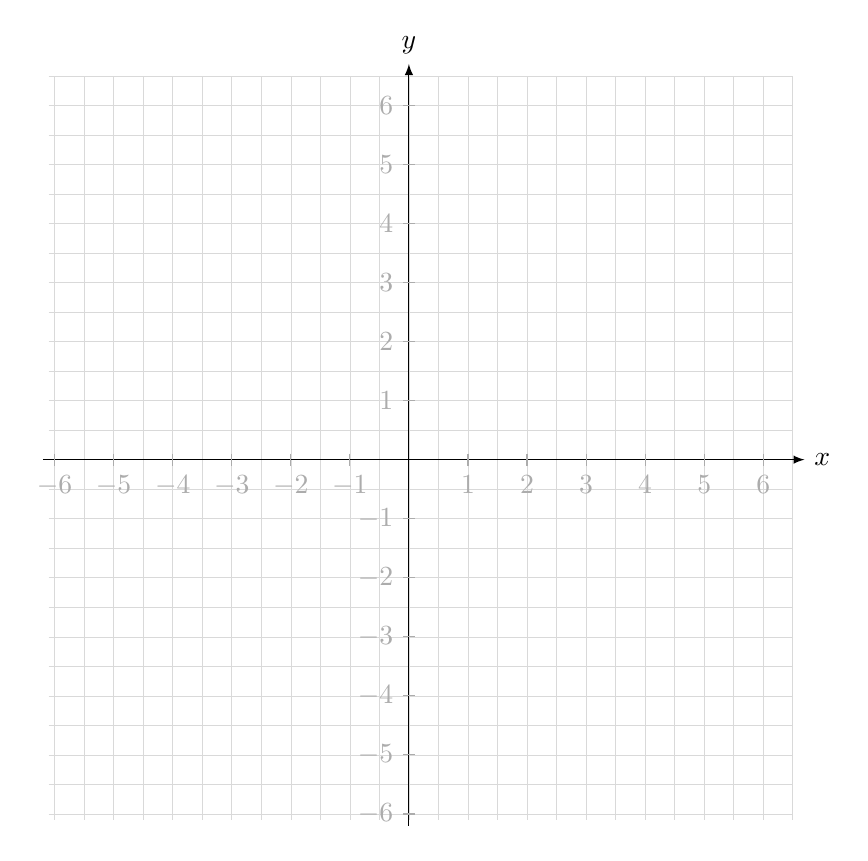
\begin{tikzpicture}[scale=0.75]
		\draw[very thin,color=black!15,step=.5] (-6.1,-6.1) grid (6.5,6.5);
		\draw[-latex] (-6.2,0) -- (6.7,0) node[right] {$x$};
		\draw[-latex] (0,-6.2) -- (0,6.7) node[above] {$y$};
		\foreach \i in {-6,...,-2,-1,1,2,...,6}
		\draw[gray!65] (\i,.1)--(\i,-.1) node[below] {$\i$};
		\foreach \i in {-6,...,-2,-1,1,2,...,6}
		\draw[gray!65] (.1,\i)--(-.1,\i) node[left] {$\i$};
	\end{tikzpicture}
\end{enumerate}
\end{tcolorbox}

\newpage
\noindent \centering Blank page \thepage~for additional work
\newpage
